\section{Design}

\subsection{Design delle Interfacce Utente}
\label{design delle interfacce utente}

In questa sezione si conclude l'analisi della \emph{Human Computer Interaction} (HCI), iniziata durante l'identificazione delle Personas precedenti.

Nelle applicazioni web è consono seguire un approccio di design \emph{mobile first} per progettare le interfacce utente, e così è stato fatto. In particolare, il \emph{progressive enhancement} dell'applicazione si è fermato proprio a livello mobile, cioè non sono stati aggiunti ulteriori raffinamenti significativi per i dispositivi desktop, poiché l'applicazione ed il gioco in sè, sono due elementi talmente minimali, in cui tutto quello da disporre nell'interfaccia è esposto in maniera ottimale anche nei dispositivi mobile.

Questo fattore non esclude il fatto che l'applicazione dispone di \emph{responsive design} e \emph{layout liquido}, ovvero, nonostante l'interfaccia dell'applicazione risulta praticamente identica in tutti i dispositivi, in realtà essa è più fruibile e più "confortevole" nei dispositivi desktop, in quanto gli elementi dell'interfaccia sono disposti su un viewport più largo e si adattano ad esso, migliorando la \emph{user experience} e l'\emph{usabilità} dell'applicazione. Un esempio: nei dispositivi mobile per leggere le regole del gioco bisogna scrollare a fondo, mentre nei dispositivi desktop è sufficiente scrollare meno. Un altro esempio: nei dispositivi desktop, i bastoncini sono renderizzati con una qualità di immagine migliore.

Qui di seguito sono rappresentati i \emph{mockup} prodotti durante la fase di design delle interfacce utente. Per contestualizzarli in relazione all'\emph{usabilità} dell'applicazione, sono stati raggruppati in due principali \emph{storyboard}.

I \emph{mockup} sono stati realizzati tramite Pencil, il quale dispone di feature per creare mockup interattivi (inter-page linking\cite{pencil_website}), ma non dispone di feature per creare \emph{storyboard}, per cui quelle inserite qui di seguito sono state prodotte con un editor generico per immagini.

La \emph{storyboard} in figura \ref{fig:storyboard - user session} rappresenta l'insieme di task inerenti alla gestione dei dati dell'utente. Mentre la \emph{stroryboard} in figura \ref{fig:storyboard - game task} rappresenta il task che svolge un utente per creare e giocare una partita.

Un approccio piuttosto informale, ma allo stesso tempo molto pratico per valutare l'\emph{usabilità} del design delle interfacce, consiste nell'osservare l'applicazione nell'ottica delle \emph{euristiche di Nielsen}. Svolgendo questa analisi, si ritiene che tutte le euristiche siano pienamente soddisfatte, soprattutto grazie al fatto della semplicità del sistema modellato.

Osservando le due \emph{storyboard} in figura \ref{fig:storyboard - user session} e \ref{fig:storyboard - game task}, si intuisce che le rotte dell'applicazione appartengono a due categorie principali: al dominio dei dati utente, oppure al dominio di gioco. Queste due categorie sono molto importanti, perché sono state sfruttate per modularizzare il design e il codice in molteplici punti.

\newpage

\begin{figure}[H]
	\centering
	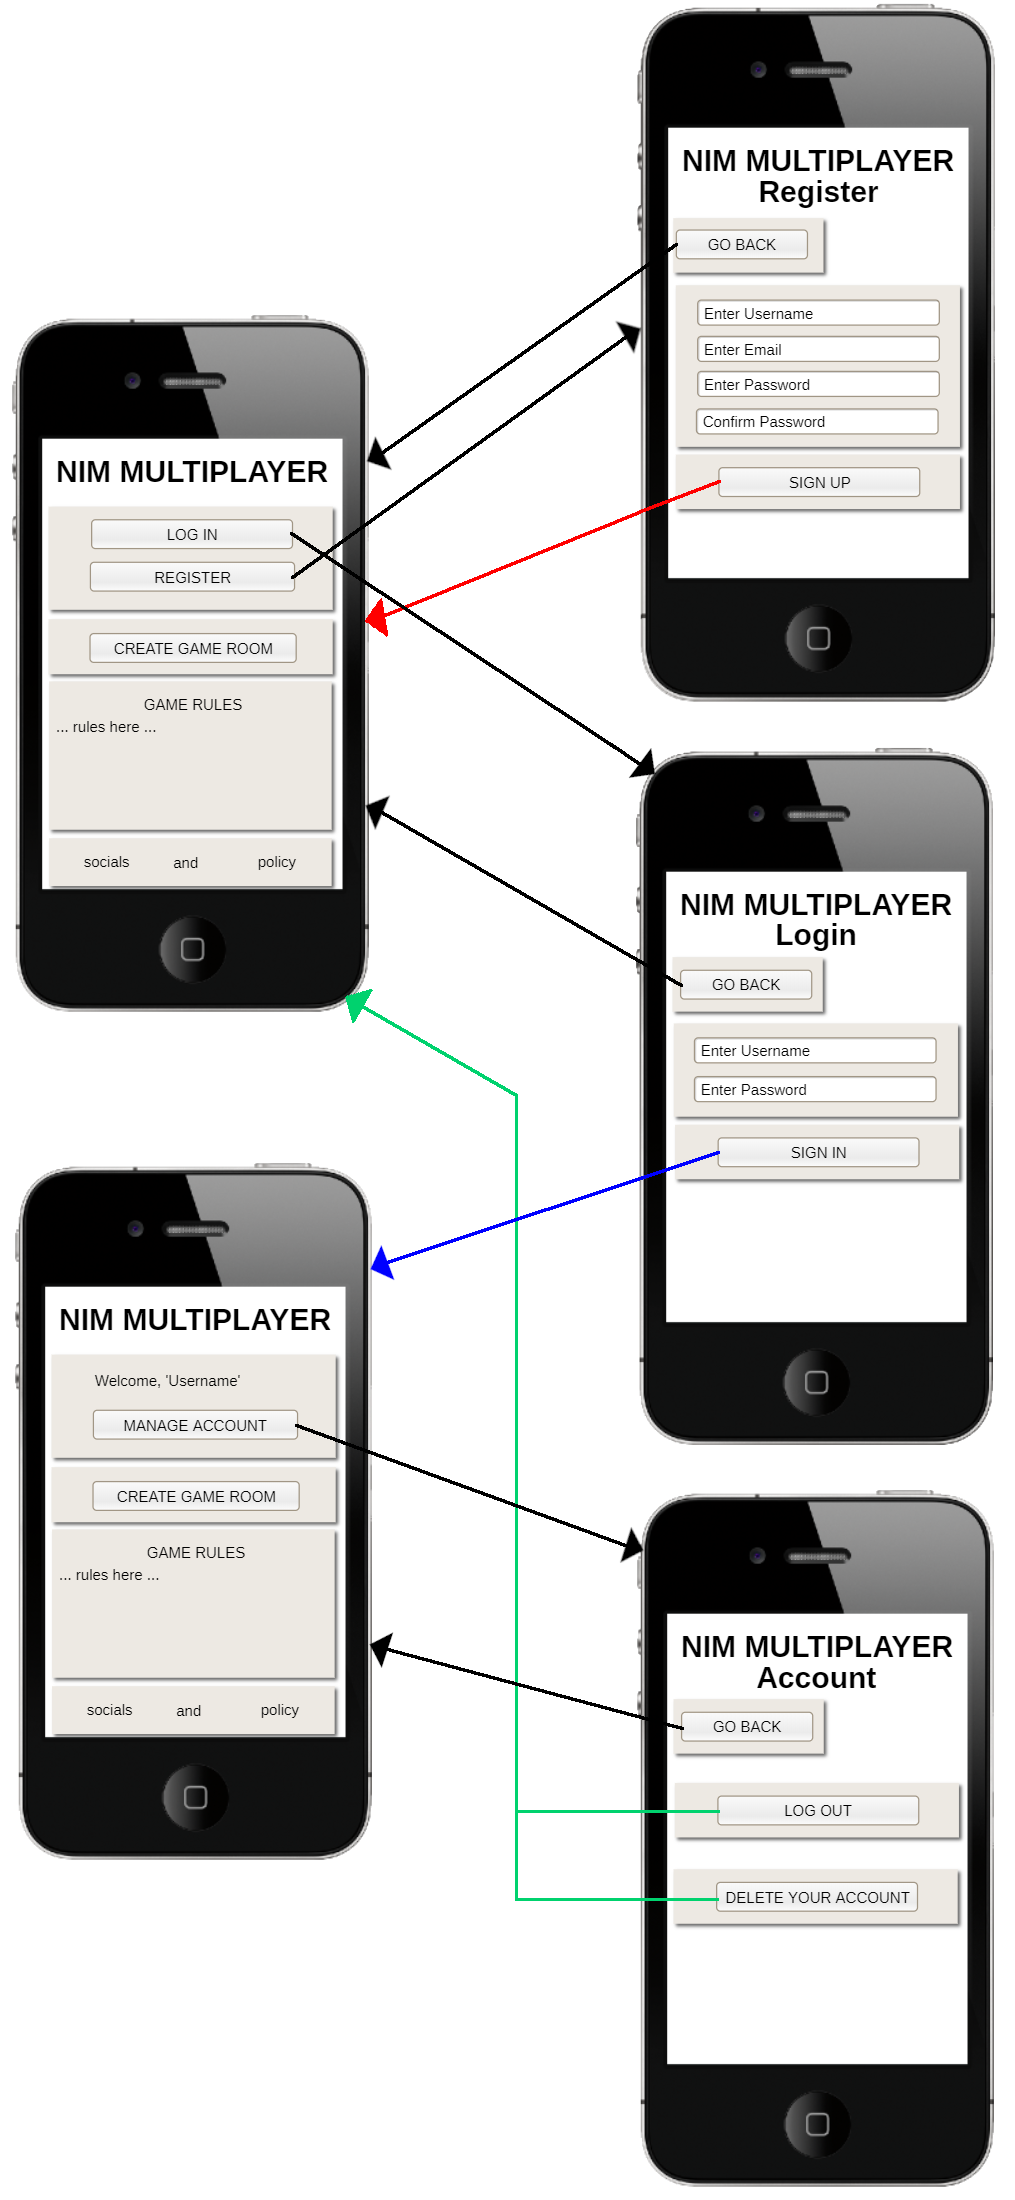
\includegraphics
	[width=0.65\linewidth]
	{storyboard with mockup - user session}
	\caption{storyboard con i mockup per gestire il dominio dei dati utente.
		\newline
		Linee nere: navigazione che non causa alcuna modifica al sistema.
		\newline
		Linea rossa: registrazione di un nuovo account utente.
		\newline
		Linea blu: login di un utente.
		\newline
		Linee verdi: logout e/o eliminazione dell'account.
	}
	\label{fig:storyboard - user session}
\end{figure}

\newpage

\begin{figure}[H]
	\centering
	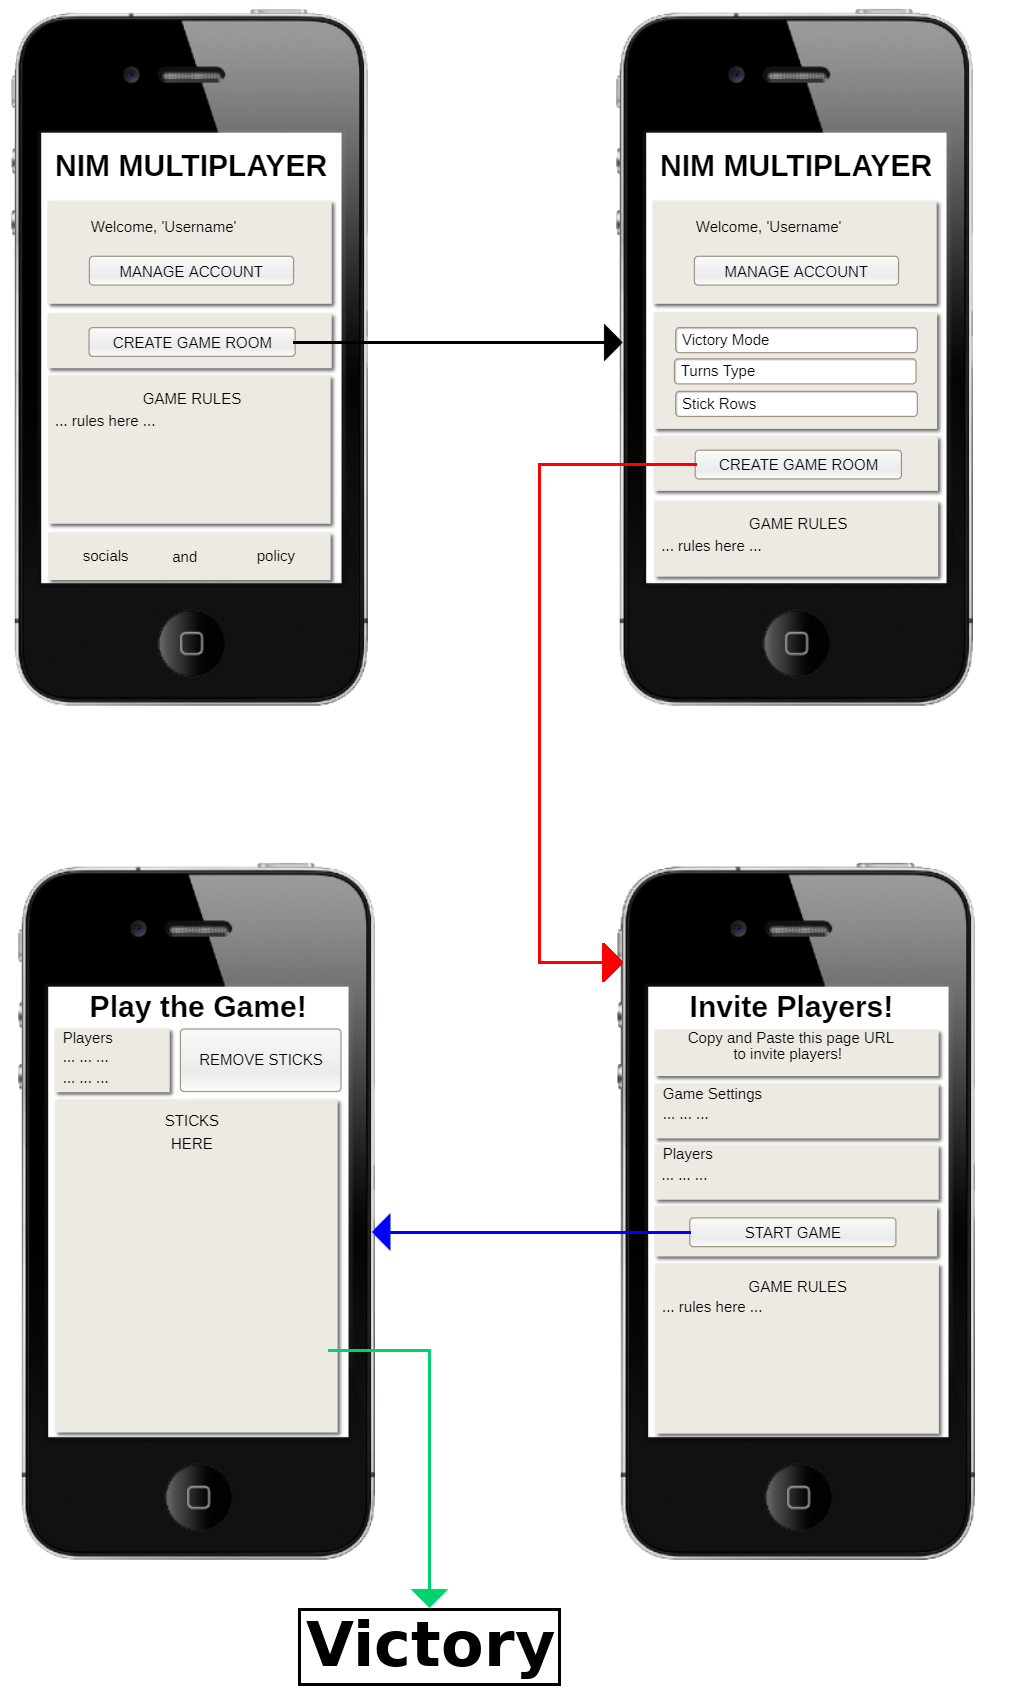
\includegraphics
	[width=0.66\linewidth]
	{storyboard with mockup - play the game}
	\caption{storyboard con i mockup per gestire la creazione e lo svolgimento di una partita (dominio di gioco).
		\newline
		Linea nera: navigazione che non causa alcuna modifica al sistema.
		\newline
		Linea rossa: creazione di una partita.
		\newline
		Linea blu: dopo aver invitato i giocatori desiderati, la partita comincia.
		\newline
		Linea verde: dopo aver giocato la partita, i giocatori sono indirizzati verso la pagina che indica il vincitore.
	}
	\label{fig:storyboard - game task}
\end{figure}

\newpage

Nella figura \ref{fig:storyboard - game task} si può osservare che il numero di giocatori non deve essere specificato prima di creare una nuova partita, bensì viene dedotto automaticamente in base a quanti utenti visitano la pagina della stanza di gioco. In questo modo, l'utente non deve scegliere il numero di giocatori, ma deve solo copiare l'URL della stanza di gioco ed inviarlo ai giocatori. Naturalmente, nella fase in cui vengono invitati i giocatori, in pagina deve essere riportato il numero massimo di giocatori che possono essere contenuti in una stanza di gioco.

\subsection{Design dell'Architettura di Sistema}

Il sistema da realizzare non richiede la gestione di situazioni particolarmente vincolanti, per questo si è scelto di adottare una soluzione di tipo \emph{Single Page Application} (SPA), al fine di ottimizzare la reattività dell'applicazione.

Di conseguenza, il layer della struttura HTML e il layer di presentazione CSS (quindi tutto ciò che riguarda la view di sistema) sono collocati totalmente a client side, mentre invece il layer di \emph{application logic} (o \emph{business logic}) è distribuito tra client e server.

\subsubsection{Front-end}
\label{design architettura - front-end}

Cercando di astrarre quanto più possibile dalle tecnologie utilizzate, la struttura della SPA deve essere organizzata nel seguente modo.

\begin{figure}[H]
	\advance\leftskip-1.2cm
	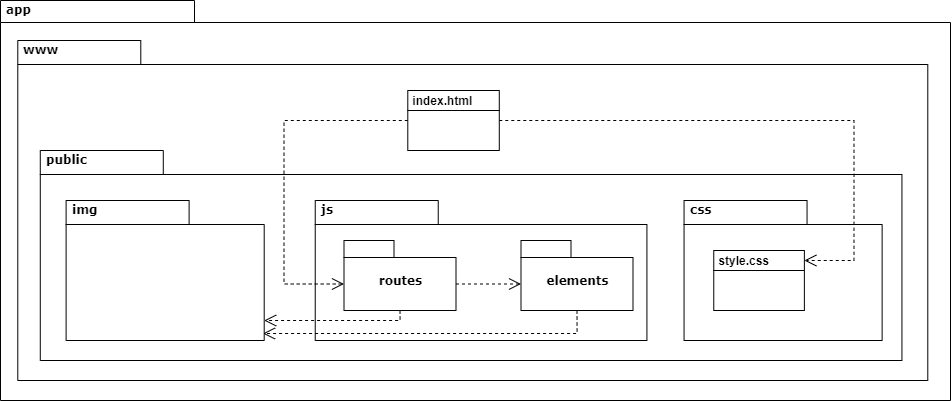
\includegraphics
	[width=1.2\linewidth]
	{package diagram - SPA}
	\caption{package diagram della SPA (la view situata a client side).
		\newline
		Per applicare maggiore chiarezza, il formalismo del package diagram è stato violato e sono stati inseriti i due file \texttt{index.html} e \texttt{style.css}, ma concettualmente il diagramma rappresenta comunque l'organizzazione e la dipendenza dei package e dei due file rappresentati.}
	\label{fig: package diagram - SPA}
\end{figure}

\newpage

\begin{enumerate}
\item
	Il file \texttt{index.html} è la \emph{Single Page}, la quale contiene al suo interno tutti gli import e la logica di \emph{Application}, quindi contiene tutti i framework o librerie e i file utilizzati a client side.
\item
	Il package \texttt{public} contiene tutti gli elementi importati ed utilizzati in \texttt{index.html}. Quindi \texttt{public} contiene l'implementazione dell'applicazione client side, e deve essere strutturato in questo modo.
	\begin{itemize}
	\item
		Il package \texttt{img} contiene le immagini.
	\item
		Il package \texttt{js} (Javascript) contiene gli elementi del framework che implementa la SPA, e deve avere a sua volta 2 sub-package.
		\begin{enumerate}
		\item
			Il package \texttt{routes} che contiene gli elementi che rappresentano le rotte (pagine) dell'applicazione.
		\item
			Il package \texttt{elements} che contiene gli elementi che rappresentano porzioni di HTML incapsulate e riutilizzate fra le rotte.
		\end{enumerate}
	\item
		Il package \texttt{css} contiene solo il file \texttt{style.css}, che rappresenta il layer di presentazione da importare in \texttt{index.html}.
	\end{itemize}
\end{enumerate}

Considerando ciò che è emerso dalla sezione \ref{design delle interfacce utente}, il package \texttt{public/js/routes} deve avere due sub-package per racchiudere i due domini presenti nel sistema: \texttt{routes/user} contiene le rotte del dominio dei dati utente; \texttt{routes/game} contiene le rotte del dominio di gioco.

\newpage

\subsubsection{Back-end}

Cercando di astrarre quanto più possibile dalle tecnologie utilizzate, la struttura del codice a server side deve essere organizzata nel seguente modo.

\begin{figure}[H]
	\advance\leftskip-1.2cm
	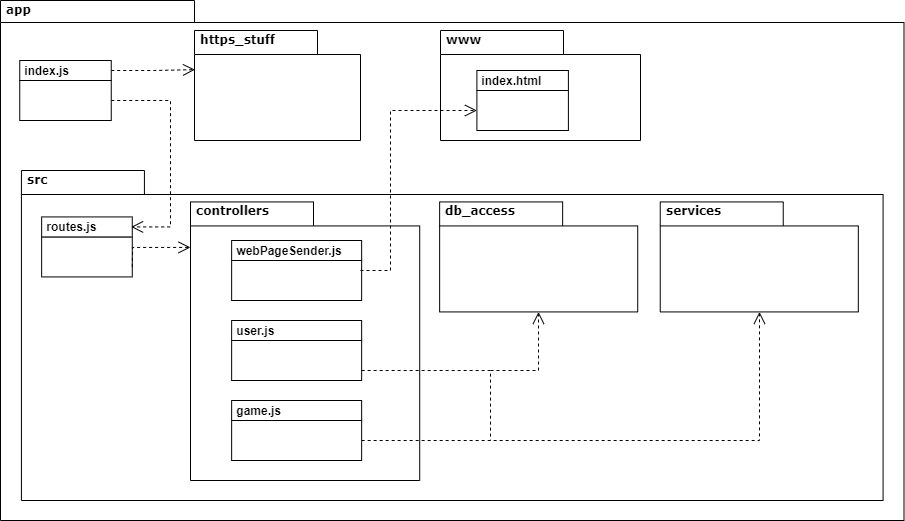
\includegraphics
	[width=1.2\linewidth]
	{package diagram - Server Side}
	\caption{package diagram dell'organizzazione server side.
		\newline
		Per applicare maggiore chiarezza, il formalismo del package diagram è stato violato e sono stati inseriti alcuni file, ma concettualmente il diagramma rappresenta comunque l'organizzazione e la dipendenza dei package e dei file rappresentati (i file rappresentati hanno estensione \texttt{js}, perché il progetto Nim Multiplayer è realizzato con la piattaforma Node e quindi è scritto in Javascript, ma a prescindere dal linguaggio usato, l'organizzazione di progetto deve essere questa).}
	\label{fig: package diagram - server side}
\end{figure}

\begin{enumerate}
\item
	Il file \texttt{index.js} è l'entry point dell'applicazione (il file eseguibile principale): connette l'applicazione al database; inizializza librerie e servizi dell'applicazione web; avvia il server.
\item
	Questo progetto adotta il pattern MVC nel web, per cui i controller agiscono tramite le rotte dell'applicazione, quindi il file \texttt{routes.js} definisce le funzionalità di sistema ed utilizza i controller per soddisfare le richieste.
\item
	Considerando quanto espresso fino ad ora, sono state individuate le responsabilità sottostanti, e ciascuna di esse è stata mappata da un corrispettivo controller rappresentato in figura \ref{fig: package diagram - server side}.
	\begin{itemize}
		\item
		Inviare la SPA verso il client che contatta il server
		\newline
		(\texttt{controllers/webPageSender.js}).
		\item
		Gestire il dominio dei dati utente, tramite chiamate Axios
		\newline
		(\texttt{controllers/user.js}).
		\item
		Gestire il dominio del gioco, tramite chiamate Axios e Socket.IO
		\newline
		(\texttt{controllers/game.js}).
	\end{itemize}
	(In figura \ref{fig: package diagram - server side} sono rappresentati tutti i controller di sistema.)
\item
	Infine, in figura \ref{fig: package diagram - server side} sono rappresentati i package sottostanti.
	\begin{itemize}
	\item
		\texttt{https\_stuff}: contiene il certificato e la chiave https.
	\item
		\texttt{db\_access}: considerando il pattern MVC, contiene gli elementi che rappresentano i model, cioè i file che accedono al database.
	\item
		\texttt{services}: contiene i file che forniscono ulteriori servizi, ad esempio: \texttt{services/user/passwordEncryption.js}.
	\end{itemize}
	Come già ribadito più volte, il sistema modella 2 domini distinti, gli utenti e il gioco, per cui \texttt{db\_access} e \texttt{services} contengono a loro volta i 2 sub-package \texttt{user} e \texttt{game} per migliorare l'organizzazione del codice.
\end{enumerate}

\paragraph{Accesso alla Persistenza: directory \texttt{db\_access} e directory \texttt{db\_access/models} \paragraphNewline}

\removeHorizontalSpaceSmall Un'importante scelta di design coinvolge la directory \texttt{app/src/db\_access} e la sua sub-directory \texttt{db\_access/models}. La directory \texttt{db\_access/models} deve contenere i modelli che rappresentano le entità salvate nel database, mentre la directory \texttt{db\_access} deve contenere gli oggetti che dispongono di metodi per manipolare tali entità ed operare sul database.
\newline
In questo modo, il codice risulta notevolmente leggibile e flessibile, ovvero le dipendenze della libreria utilizzata per interfacciarsi al database, sono totalmente incapsulate dentro i file di \texttt{db\_access}, per cui si può cambiare tecnologia di interfacciamento al database, semplicemente modificando i file di \texttt{db\_access} e di \texttt{db\_access/models}.
\newline
Un esempio di codice per comprendere questi vantaggi è riportato in \ref{persistenza: db_access - Codice}.

Questa organizzazione di codice appena descritta, è una sorta di pattern adapter\footnote{Adapter design pattern, descritto in GoF\citep{GoF}.}, in cui l'adaptee è la libreria scelta per interfacciarsi al database e gli adapter sono gli oggetti di \texttt{db\_access}.

Un altro esempio strutturalmente identico a questo tipo di pattern adapter, è osservabile nel file \texttt{app/src/services/user/passwordEncryption.js}, quest'ultimo adatta (seppur in maniera estremamente minimale) la libreria scelta per cifrare e decifrare la password nel database.

\newpage

\paragraph{Persistenza: Dati degli Utenti \paragraphNewline}

\removeHorizontalSpaceSmall Per memorizzare i dati degli utenti, è sufficiente disporre uno spazio di archiviazione che ammette solamente una tipologia di dato omogenea. I dati degli utenti memorizzati sono sempre gli stessi per ogni utente: l'identificativo (cioè l'username); la password; l'email (che è un secondo identificativo).

\paragraph{Persistenza: Stato delle Partite \paragraphNewline}

\removeHorizontalSpaceSmall Per memorizzare lo stato delle partite è assolutamente consigliato l'impiego di una tecnologia di persistenza NoSQL, perché il numero dei bastoncini e il numero di giocatori sono valori variabili per ogni partita (ma non solo, vi sono anche altri valori illustrati qui di seguito che sono variabili), pertanto NoSQL permette di gestire queste caratteristiche dinamiche con facilità.

Un dettaglio interessante inerente alla memorizzazione delle partite, è che indipendentemente dalla loro configurazione, il loro schema è sempre lo stesso, sia che una partita abbia modalità di vittoria Standard o Marienbad, sia che una partita abbia i turni in rotazione oppure chaos.

I dati memorizzati all'interno di uno schema di una partita sono riportati nel seguente elenco, e per ognuno di essi viene descritto come il loro valore influenza il comportamento di gioco.
\begin{itemize}
\item
	\texttt{sticks}: rappresenta i bastoncini, è un dato variabile per ogni partita, ed è rappresentato come una matrice, cioè un array di array in cui quest'ultimi sono le righe che contengono i valori dei bastoncini.
	\newline
	I valori dei bastoncini sono impostati inizialmente a false, e questo rappresenta lo stato di "bastoncino rimosso = false". Per gestire tutte le casistiche di configurazione di una partita, quando un bastoncino viene rimosso, nel valore del bastoncino viene inserito il nome del giocatore che lo ha rimosso. In questo modo, nelle partite Marienbad multiplayer, quando un giocatore viene eliminato, si possono facilmente ripristinare tutti i bastoncini rimossi dai giocatori presenti in gioco (come richiesto in \ref{requisiti funzionali}).
	\newline
	(Nel caso di una partita con modalità di vittoria Standard multiplayer, o nel caso di una partita 1 vs 1, sarebbe sufficiente inserire true come valore nei bastoncini rimossi, ma per semplicità si è scelto di adottare la soluzione appena descritta per soddisfare i vincoli di tutte le tipologie di partite.)
\item
	\texttt{standardVictory}: rappresenta la modalità di vittoria, è un valore booleano, \texttt{true} significa che la partita ha vittoria Standard, \texttt{false} significa che la partita ha vittoria Marienbad.
\item
	\texttt{turnRotation}: rappresenta la rotazione dei turni, è un valore booleano, \texttt{true} significa che i turni sono in rotazione, \texttt{false} significa che i turni sono chaos.
\item
	\texttt{activePlayer}: è una stringa che contiene l'username del giocatore di turno.
\item
	\texttt{players}: è un array con dimensione variabile che contiene gli username degli utenti in partita.
	\newline
	Il suo significato cambia in base alla modalità di rotazione dei turni.
	\begin{itemize}
	\item
		se \texttt{turnRotation} è uguale a \texttt{true}, allora i turni dei giocatori sono alternati per tutta la partita, seguendo l'ordine di \texttt{players}, generato casualmente ad inizio partita.
	\item
		se \texttt{turnRotation} è uguale a \texttt{false} (turni chaos), allora \texttt{players} contiene i giocatori che devono svolgere il turno. Quando un giocatore svolge il suo turno, viene inserito in \texttt{playersWithTurnDone}. Quando \texttt{players} è vuoto e \texttt{playersWithTurnDone} contiene tutti i giocatori, allora tutti i giocatori vengono rimossi da \texttt{playersWithTurnDone} per essere inseriti dentro \texttt{players}.
	\end{itemize}
\item
	\texttt{playersWithTurnDone}: è un array con dimensione variabile che contiene gli username degli utenti che hanno svolto il proprio turno.
	\newline
	Questo dato viene utilizzato solo nelle partite con turni chaos.
\item
	\texttt{eliminatedPlayers}: è un array con dimensione variabile che contiene gli username degli utenti eliminati dalla partita.
\item
	\texttt{disconnectedPlayers}: è un array con dimensione variabile che contiene gli username degli utenti disconnessi, e che devono essere eliminati dalla partita nel momento in cui si presenta il loro turno.
\end{itemize}

\subsubsection{Front-end vs Back-end}
\label{front-end vs back-end}

In tutte le applicazioni web, si deve cercare di spostare quanto più possibile l'application logic a client side, in modo da ridurre il carico di lavoro del server.

\paragraph{Rotte del Dominio dei Dati Utente \paragraphNewline}

\removeHorizontalSpaceSmall Per il motivo appena descritto, nella pagina di registrazione, è la SPA che deve avere la responsabilità di eseguire i controlli riguardo l'inserimento degli input field. In seguito, il server si deve occupare di verificare che: l'username e la mail non sono dati già registrati; l'username non supera una certa lunghezza, perché altrimenti questo causa problemi di renderizzazione dell'username durante il gioco (questo controllo è stato inserito a server side, perché è stato ritenuto più "sicuro" svolgerlo lì).

Allo stesso modo, nella pagina di login, è la SPA che deve avere la responsabilità di eseguire i controlli riguardo l'inserimento degli input field. In seguito, il server si deve occupare di svolgere i controlli sul database.

\paragraph{Rotta della Stanza di Gioco \paragraphNewline}

\removeHorizontalSpaceSmall Sempre per lo stesso motivo, nella pagina di gioco, è la SPA che deve avere la responsabilità di validare la mossa prima di inviarla al server. In seguito, il server si deve occupare di applicare la mossa alla partita, e gestire le disconnessioni dei giocatori in caso si verifichino.

\newpage